\section{Parallelisation}
\label{parallel}
\indent
\par 

\subsection{Sequential Profiling}
Prior to parallelisation every step of the linear algebra expression was profiled in order to identify potencial hotspots. Since in the later sections, the best parallel linear algebra version turned out to be the CSC version, special attention is added to it when compared to the CSR version. \par 
Table \ref{table:profile_seq} demonstrates the profiler results, namely the percentage of overall time for each of the operation present in expression \ref{eq:tpch_1}, for the CSC version, for the largest TPC-H dataset in test - 32GB.

\begin{table}[H]
\centering
\footnotesize
  \begin{tabular}{ | L{1cm} | L{1.25cm} |  L{1.2cm} |  L{1.3cm} |  L{1.6cm} | L{1cm} |  }
    \hline
    LA Version	&	Projection	&	Selection	&	Projection . Selection	&	(Projection .Selection). Quantity	&	Bang	\\ \hline
Seq. CSC	&	23.93\%	&	43.38\%	&	10.89\%	&	18.12\%	&	3.68\%	\\ \hline
  \end{tabular}
     \caption{Profiling results for the sequential CSC linear algebra version, for TPC-H 32GB dataset, for the evaluation platform.}
     \label{table:profile_seq}
\end{table}

As you can observe  on table \ref{table:profile_seq}, the most time consuming operations are the Selection and the Projection (Khratri-Rao operation). Further efforts will be made in order to reduce the selection overhead in the later subsection \ref{optimization_selection}. \par 

\subsection{Parallel Experimental Results and Analysis}

To parallelise both linear algebra versions, OpenMP version 4.0 was used.
Based on the CSC Sparse Format linear algebra version, since each column has at most one element, the used algorithms give place to good parallelisation opportunities. Regarding the CSR format the used algorithms present more challenging parallel  optimisations. \par 

Figure \ref{fig:time_la_vs_ra_parallel} presents the measured time analysis regarding the variety of datasets, the test platform, and both linear and relational algebra approaches. Denote that the presented values were selected through the K-Best technique, with K=3 from a 50 samples. Regarding the linear algebra approach we present the the best solution from CSR and CSC format, namely the CSC format version.\par
As visible, the parallel linear algebra solution surpasses the parallel relational algebra, however larger TPC-H datasets reduce the gain from the linear algebra approach. Further algorithm optimisation will be analysed in the following subsection \ref{optimization_selection}.\par 

\begin{figure}[H]
\centering
\caption{TPC-H benchmark simplified query-1 time for solution analysis for different scale factors, between parallel linear and relational algebra approaches.}
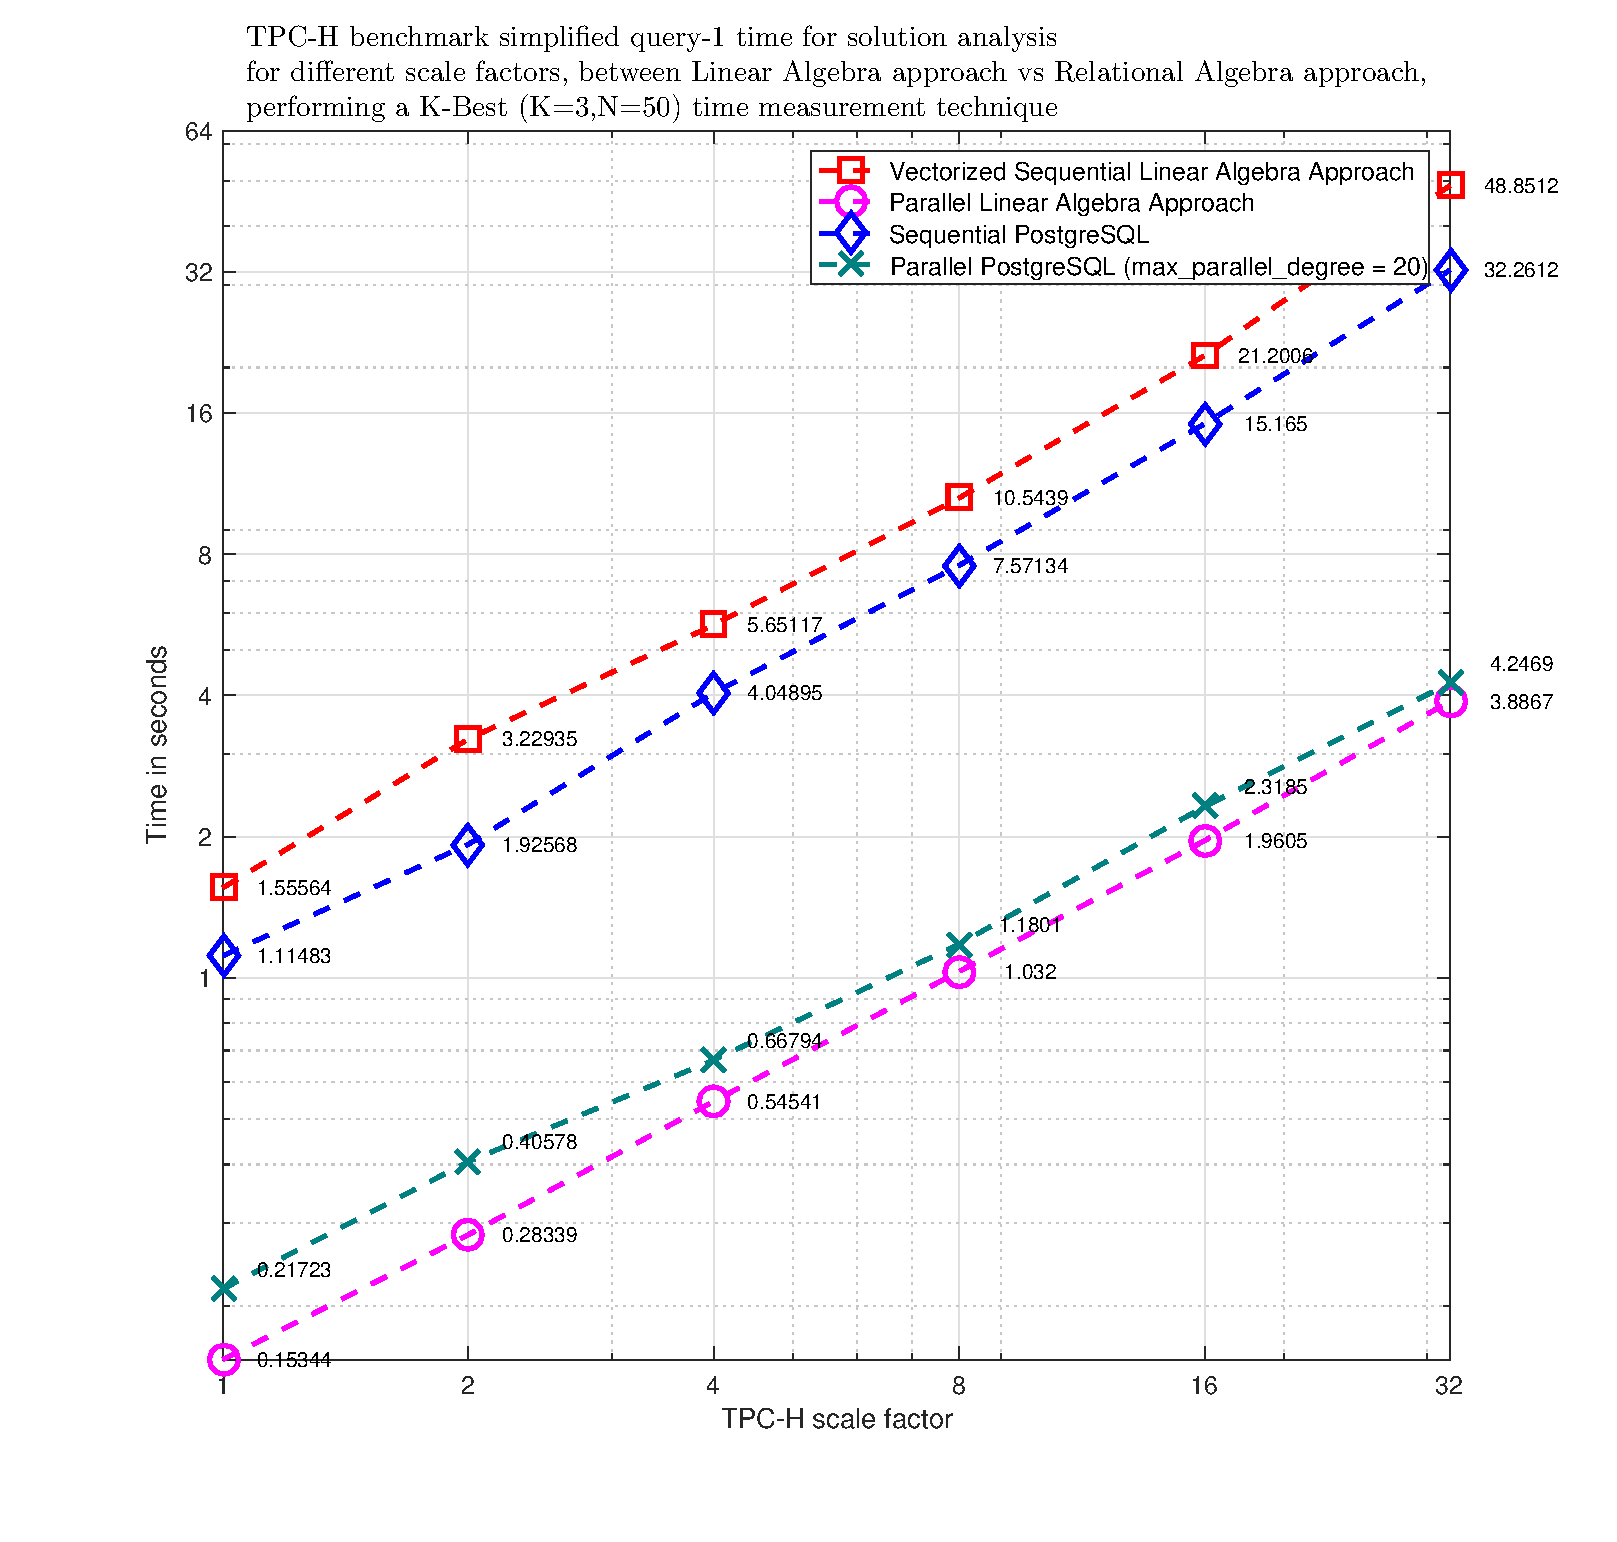
\includegraphics[width=1\columnwidth]{eps/TIME_LA_vs_RA_parallel.eps}
\label{fig:time_la_vs_ra_parallel}
\end{figure}

\subsection{Further Selection Algorithm Optimisation}
\label{optimization_selection}

Further profiling was made in order to fully examine the potential bottlenecks. Table \ref{table:profile_par} compares both sequential and parallel linear algebra versions. As you can observer the Projection operation has diminished the percentage of overall time to complete the operation. However the Selection operation has increased its percentage overall time to almost half the time. \par 


\begin{table}[H]
\centering
\footnotesize
  \begin{tabular}{ | L{1cm} | L{1.25cm} |  L{1.2cm} |  L{1.3cm} |  L{1.6cm} | L{1cm} |  }
    \hline
    LA Version	&	Projection	&	Selection	&	Projection . Selection	&	(Projection .Selection). Quantity	&	Bang	\\ \hline
Seq. CSC	&	23.93\%	&	43.38\%	&	10.89\%	&	18.12\%	&	3.68\%	\\ \hline
Par. CSC	&	13.62\%	&	46.83\%	&	11.49\%	&	16.74\%	&	3.51\%	\\ \hline

  \end{tabular}
     \caption{Profiling results for the parallel CSC linear algebra version, for TPC-H 32GB dataset, for the evaluation platform.}
     \label{table:profile_par}
\end{table}

After a careful examination of a portion the C source code for the CSC version selection, presented on listing \ref{selection_code_old}, further algorithm optimisations can be made. 

\lstinputlisting[caption=portion of the C source code for the CSC linear algebra version selection algorithm, label=selection_code_old]{src/selection_old.c} 

Taking as example the TPC-H 32GB dataset, and the shipdate matrix, with dimension $(\ m\ \times\ n\ ), namely $(\ 2531\ $\times\ 192000551\ )$, to compute the selection result, in the worst case scenario, it is necessary to realize $(n * 2) = 384001102 $ string comparisons. However, by analysing table \ref{table:dataset_info}, you can denote that from the 384001102 string comparisons only 2531 strings will be tested.\par 
 Listing \ref{selection_code_new} avoids repetitive string comparisons  adding and additional auxiliar array (of size n), resulting in a worst case scenario of  $(m * 2) = 5062 $ string comparisons and $n = 192000551 $ integer comparisons.\par
 This solution resolves two distinct problems: the first being the excessive overhead of requiring a large amount and repetitive string comparisons, and the second being the improvement of this solution with bigger datasets. The additional overhead of producing an auxiliar array gets diminished with the increase of the dataset  and consequently the required comparisons.  The bigger the dataset the better. 

\lstinputlisting[caption=portion of the C source code for the CSC linear algebra version selection algorithm, label=selection_code_new]{src/selection_new.c} 

Table \ref{table:profile_par_new} compares both sequential, parallel, and optimised parallel linear algebra versions. As you can observer the Selection operation has largely diminished its percentage overall time making it possible for the overall time to be averagely distributed among operations. \par 

\begin{table}[H]
\centering
\footnotesize
  \begin{tabular}{ | L{1cm} | L{1.25cm} |  L{1.2cm} |  L{1.3cm} |  L{1.6cm} | L{1cm} |  }
    \hline
    LA Version	&	Projection	&	Selection	&	Projection . Selection	&	(Projection .Selection). Quantity	&	Bang	\\ \hline
Seq. CSC	&	23.93\%	&	43.38\%	&	10.89\%	&	18.12\%	&	3.68\%	\\ \hline
Par. CSC	&	13.62\%	&	46.83\%	&	11.49\%	&	16.74\%	&	3.51\%	\\ \hline
Optimized Par. CSC	&	10.47\%	&	20.10\%	&	25.86\%	&	34.60\%	&	8.98\%	\\ \hline
  \end{tabular}
     \caption{Profiling results for the selection algorithm optimised parallel CSC linear algebra version, for TPC-H 32GB dataset, for the evaluation platform.}
     \label{table:profile_par_new}
\end{table}

\subsection{Final Parallel Experimental Results}

Figure \ref{fig:time_la_vs_ra_parallel_v2} presents the measured time analysis regarding the variety of datasets, the test platform, and both linear and relational algebra approaches. Denote that the presented values were selected through the K-Best technique, with K=3 from a 50 samples. 
Regarding the linear algebra approach we present the the best solution from CSC format, with the selection algorithm optimisation.\par
As visible, the parallel linear algebra solution surpasses in both versions the parallel relational algebra, and the problem regarding the reduction of gain with the increase of  TPC-H datasets was eliminated.\par 
Figure \ref{fig:speedup_la_vs_ra_parallel} states the obtained speedup between the best linear algebra version and the best relation algebra version.

\begin{figure}[H]
\centering
\caption{TPC-H benchmark simplified query-1 time for solution analysis for different scale factors, between parallel linear and relational algebra approaches, in which linear algebra approach states the selection algorithm optimisation.}
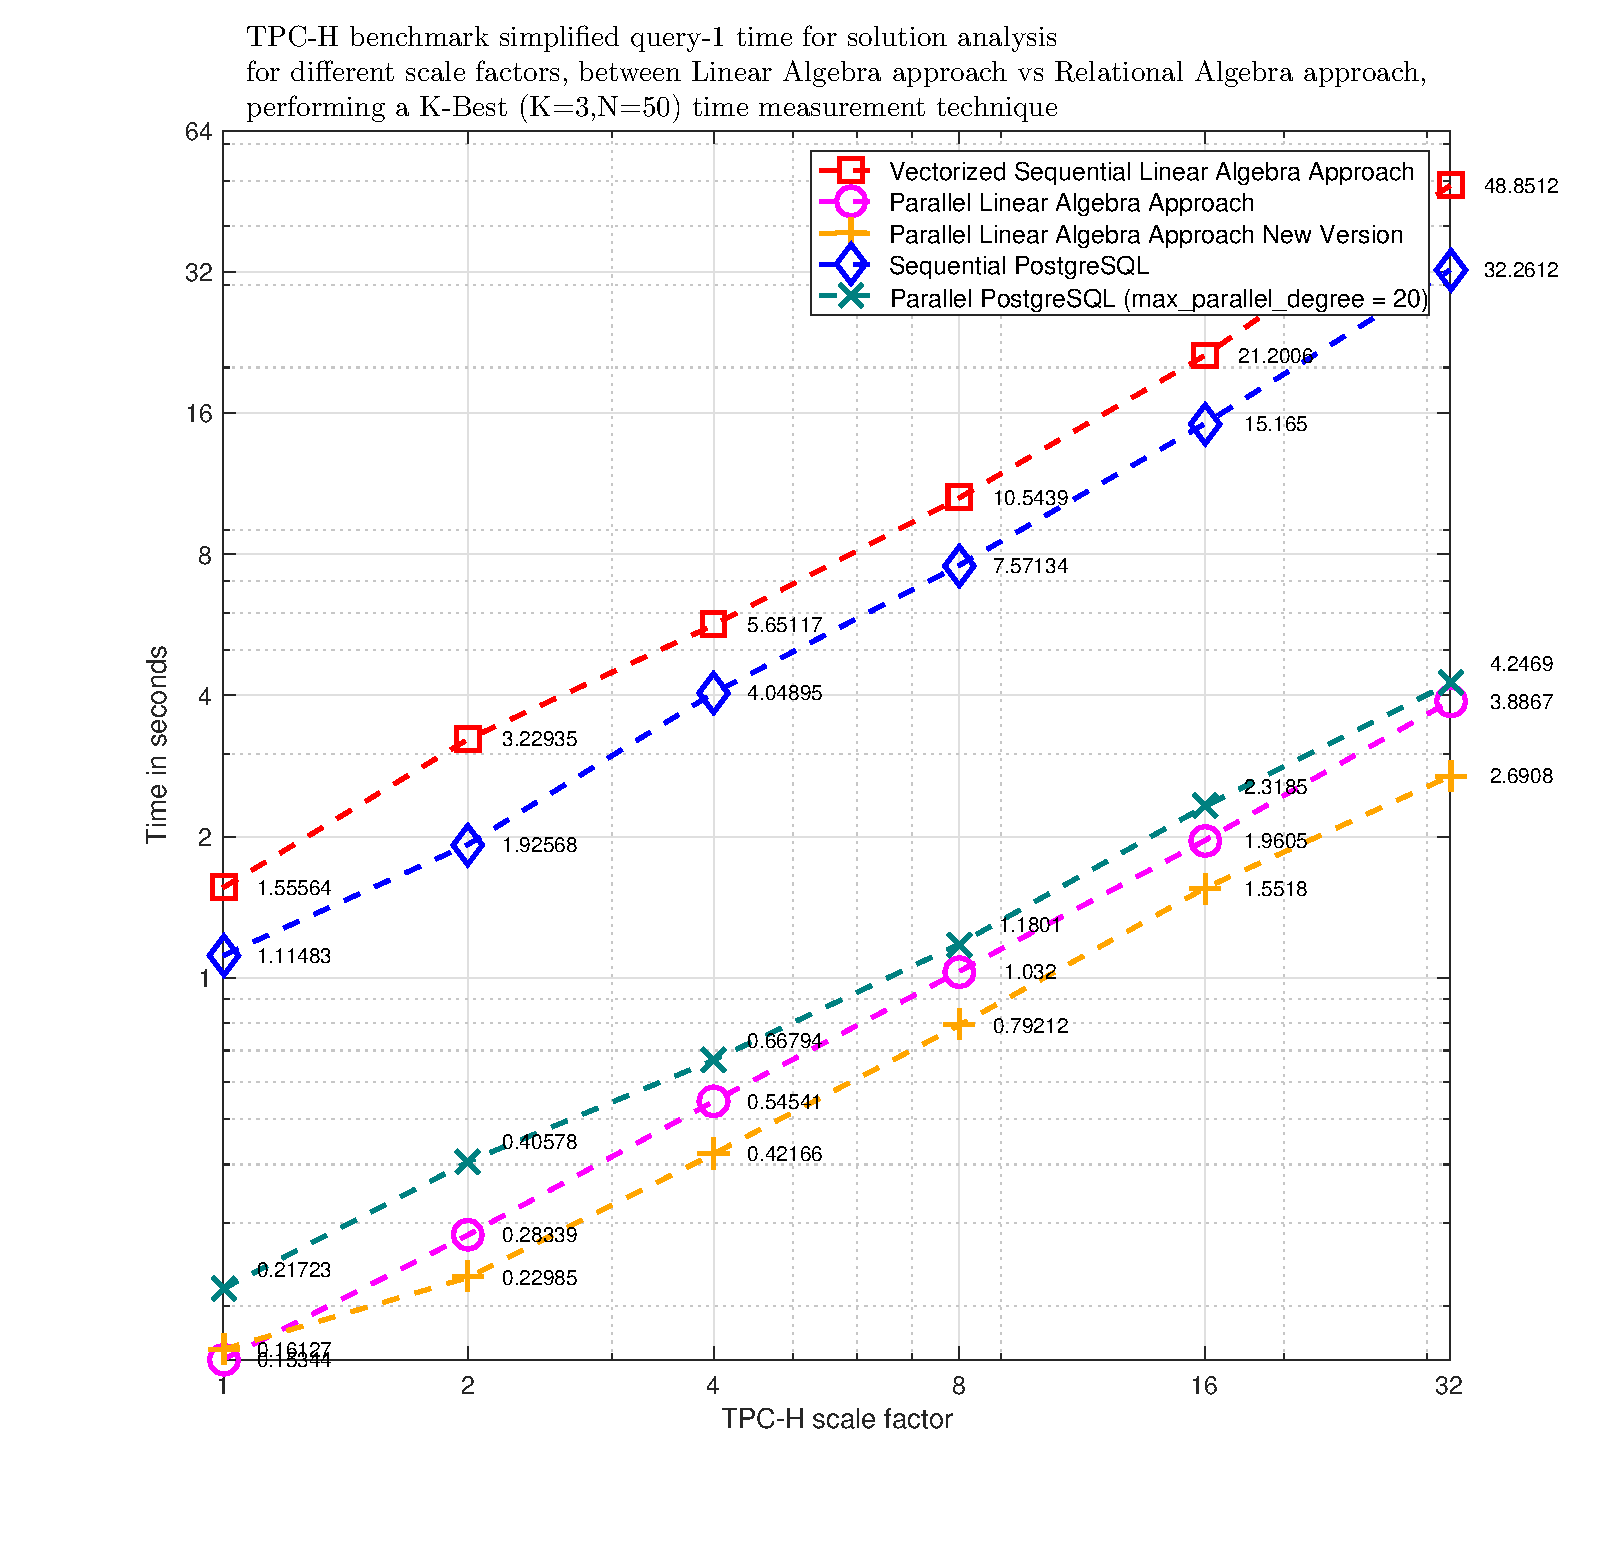
\includegraphics[width=0.95\columnwidth]{eps/TIME_LA_vs_RA_parallel_v2.eps}
\label{fig:time_la_vs_ra_parallel_v2}
\end{figure}



\begin{figure}[H]
\centering
\caption{TPC-H benchmark simplified query-1 speedup analysis for different scale factors, between sequential linear algebra vs parallel linear algebra and parallel linear algebra vs parallel relational algebra.}
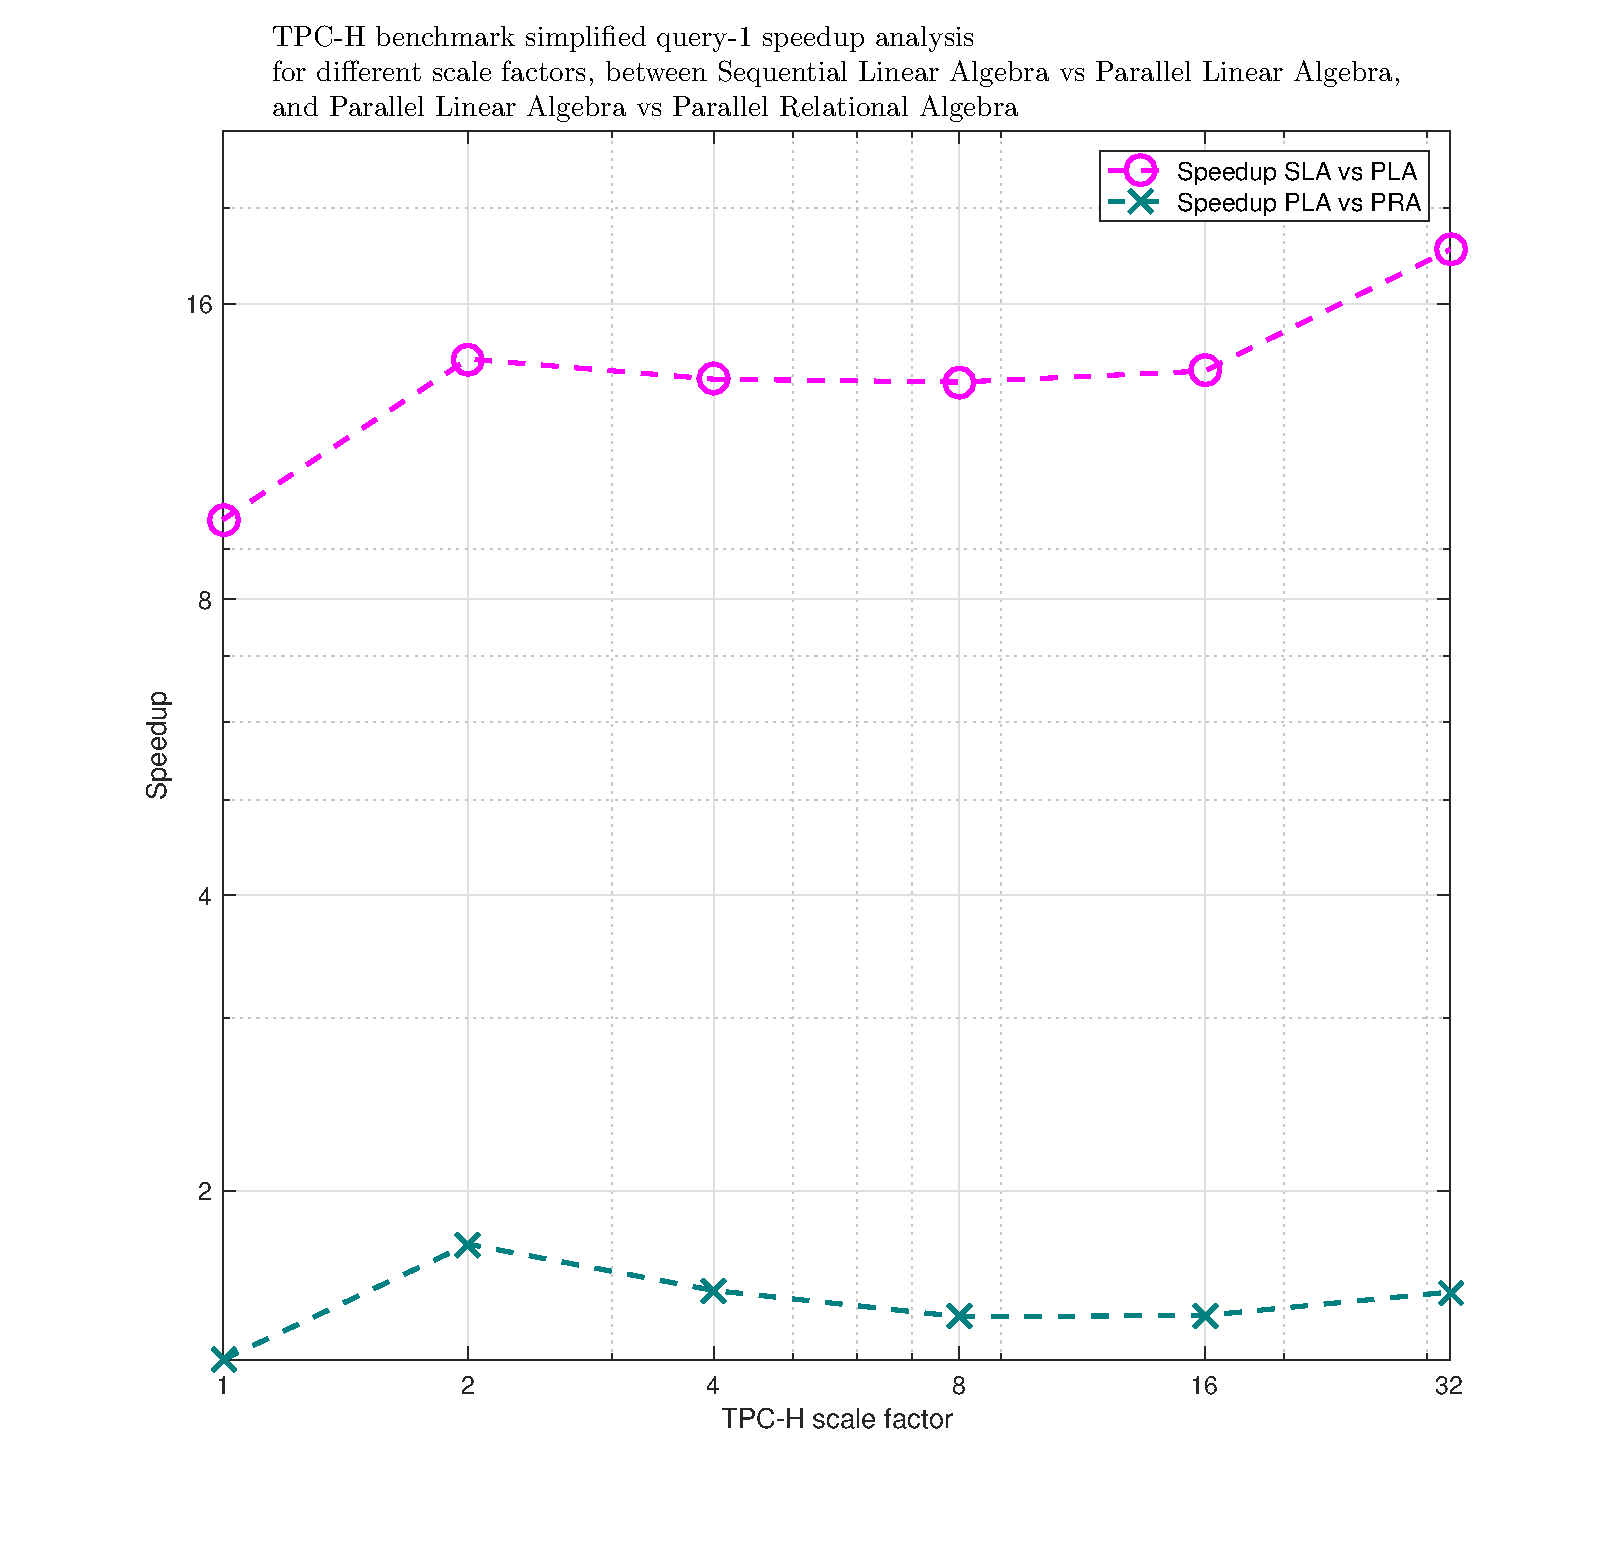
\includegraphics[width=0.95\columnwidth]{eps/speedup.eps}
\label{fig:speedup_la_vs_ra_parallel}
\end{figure}



